\documentclass[review]{elsarticle}

\usepackage{lineno,hyperref}
\modulolinenumbers[5]

\journal{Ocean Engineering }

%%%%%%%%%%%%%%%%%%%%%%%
%% Elsevier bibliography styles
%%%%%%%%%%%%%%%%%%%%%%%
%% To change the style, put a % in front of the second line of the current style and
%% remove the % from the second line of the style you would like to use.
%%%%%%%%%%%%%%%%%%%%%%%

%% Numbered
%\bibliographystyle{model1-num-names}

%% Numbered without titles
%\bibliographystyle{model1a-num-names}

%% Harvard
%\bibliographystyle{model2-names.bst}\biboptions{authoryear}

%% Vancouver numbered
%\usepackage{numcompress}\bibliographystyle{model3-num-names}

%% Vancouver name/year
%\usepackage{numcompress}\bibliographystyle{model4-names}\biboptions{authoryear}

%% APA style
%\bibliographystyle{model5-names}\biboptions{authoryear}

%% AMA style
%\usepackage{numcompress}\bibliographystyle{model6-num-names}

%% `Elsevier LaTeX' style
\bibliographystyle{elsarticle-num}
%%%%%%%%%%%%%%%%%%%%%%%

\begin{document}

\begin{frontmatter}

\title{Quantitative benchmark of a single rising bubble using VoF methods}

%% Group authors per affiliation:
\author[ifpenaddress]{Lionel Gamet\corref{mycorrespondingauthor}}
\cortext[mycorrespondingauthor]{Corresponding author}
\ead{Lionel.Gamet@ifpen.fr}
\ead[url]{www.ifpenergiesnouvelles.fr}

%% or include affiliations in footnotes:
\author[ifpenaddress]{Marco Scala}

\author[stromningaddress]{Johan Roenby}

\author[dlraddress]{Henning Scheufler}

\address[ifpenaddress]{IFPEN Lyon, Process Experimentation Division, 69360 Solaize, France}
\address[stromningaddress]{STROMNING, Luftmarinegade 62, 1432 K{\o}benhavn K, Denmark}
\address[dlraddress]{DLR German Aerospace Center, Institute of Space Systems, 28359 Bremen, Germany}

\begin{abstract}
This template helps you to create a properly formatted \LaTeX\ manuscript.
\end{abstract}

\begin{keyword}
\texttt{elsarticle.cls}\sep \LaTeX\sep Elsevier \sep template
\MSC[2010] 00-01\sep  99-00
\end{keyword}

\end{frontmatter}

\linenumbers

%%======================================================================
\section{Introduction}
%%======================================================================

Gas-liquid interfacial flow systems are often encountered in a wide variety of configurations, in science, engineering or industry. In ocean engineering, floating wind turbines, oil and gas platforms, or more generally coastal and offshore structures are submitted to violent waves, which is a paramount concern for their correct dimensioning. In the chemical process industry, various scales of gas-liquid flows are encountered ranging from large bubble columns, plate columns, agitated vessels, surface aerators, jets, static mixers or micro-reactors. Their applications are generally reactive flow systems, mixing, stripping or saturation systems. Complex phenomena of turbulent hydrodynamics involving breakup and coalescence, coupled with gas-liquid mass and heat transfers, appear in such systems. Many other applications of interfacial flows can be found. Their list would be endless, but we can cite domains like inkjet printing, automotive applications (liquid films, fuel injection, aquaplaning, ...), ship maneuvering, tank sloshing, hydraulic pumps, metal casting, fire sprinklers, atomizers, etc ... The list of domains that may benefit from improved solution methods to the interface advection problem is thus extremely large. 

Thanks to the increase of computing resources, highly resolved simulations gain more and more 
interest to analyze in detail the physics of such multiphase flows. Many numerical methods 
have emerged to attempt to simulate gas-liquid flows. Among these, implicit interface capturing 
approaches like volume of fluid (VoF)~\cite{HIRT1981201} and level set (LS)~\cite{OSHER198812} 
have proven to be efficient in simulating multiphase flows. 

Before running into complex geometries, elementary quantitative benchmark configurations are 
essential for validation and comparison of interfacial flow solvers. Hysing et 
al.~\cite{Hysing2009} have proposed a 2D benchmark consisting in a single rising bubble in 
a quiescent liquid. Two different cases are described in~\cite{Hysing2009}, corresponding to 
different density, viscosity and surface tension ratios. More recently, Adelsberger et al.~\cite{Adelsberger2014} have published a 3D equivalent of the same benchmark. For both these benchmarks, result data was made available online by the authors at the URLs mentioned in the bibliography. 

Roenby et al.~\cite{Roenby160405} have recently developed a new geometric VoF method, called isoAdvector, for advecting the interface between two incompressible fluids. This method was implemented in OpenFOAM-v1706 in the new solver \verb+interIsoFoam+. 
More recently, Scheufler and Roenby~\cite{Scheufler2018} have introduced a novel computational interface reconstruction scheme based on the calculation of a reconstructed distance function (RDF). This new scheme has been combined with the interface advection step of the isoAdvector algorithm~\cite{Scheufler2018}. Second order convergence with reduced absolute errors is obtained for simple test cases on all mesh types. The implementation of the proposed interface reconstruction scheme is straightforward and its computational cost is low. 

IsoAdvector gives a sharper interface, but validation data for this new method is still sparse, especially for surface tension dominated flows. Following the single rising bubble benchmarks~\cite{Hysing2009,Adelsberger2014}, the objective of this paper is to perform quantitative comparisons of the isoAdvector method with the benchmark data. Furthermore, the isoAdvector results are compared with results from OpenFOAM's original interfacial flow solver, \verb+interFoam+~\cite{Weller2008}.

%%======================================================================
\section{Numerical methods}
%%======================================================================
We consider here an unsteady, laminar, isothermal and incompressible two-phase flow. The flow is supposed without mass transfer across the gas-liquid interface. The governing equations are the continuity and linear momentum equations. The incompressibility condition is written as a divergence free equation for the velocity field:
\begin{equation}
  \nabla \cdot \overrightarrow{U} = 0
\end{equation}
The Navier-Stokes equations for the momentum evolution are written as: 
\begin{equation}
  \frac{\partial(\rho \overrightarrow{U})}{\partial t} + 
  \overrightarrow{\nabla} \cdot (\rho\overrightarrow{U}\overrightarrow{U}) = 
  \overrightarrow{\nabla} \cdot \left( \mu (\nabla\overrightarrow{U}+\nabla^T\overrightarrow{U})\right)
  - \overrightarrow{\nabla} p + \rho \overrightarrow{g} + \overrightarrow{F_{\sigma}}
\end{equation}
where $p$, $\rho$, $\mu$ are respectively the pressure, density and viscosity of the mixture. $\overrightarrow{U}$ denotes the velocity of the mixture. $\overrightarrow{g}$ is the gravity. $\overrightarrow{F_{\sigma}}$ represents the surface tension force, which is expressed as a source term in the momentum equation. 

In the VoF method, the continuity equation is converted into an convection diffusion equation for the volume fraction field $\alpha$, representing for each cell the fraction of its volume, which is occupied by one of the two fluids. Mixture quantities are defined as volume fraction weighted sums. If $\alpha$ denotes the first phase volume fraction, $\rho_1$ the first phase density, $\rho_2$ the second phase density, then the mixture density is defined as $\rho = \alpha\rho_1 + (1-\alpha)\rho_2$. All other mixture quantities are defined similarly. 
Special care must be taken in the numerics to prevent smearing of the $\alpha$-field and at the same time keeping it bounded ($0\leq \alpha\leq 1$). In the \verb|interFoam| solver, sharpness is obtained by introducing an artificial interface compression term in the $\alpha$-equation~\cite{Weller2008}, and boundedness is ensured by employing the MULES limiter (Multidimensional Universal Limiter with Explicit Solution). More details can be found in Deshpande~\cite{Deshpande2012}.

The solver \verb+interFoam+ has been widely used and validated~\cite{MARSCHALL2012,RAEINI2012,HOANG2013,BILGER2017}, but under some conditions the described method may fail in keeping the interface sufficiently sharp. Furthermore, the heuristic nature of the added compression term can lead to inaccurate interface advection and undesirable features such as unphysical ripples on the interface \cite{roenby_new_2017,roenby_isoadvector:_2018}. This motivated the development of the isoAdvector geometric VoF method, which was first presented by Roenby et al.~\cite{Roenby160405}. In the latter reference, it was tested with a variety of pure advection cases yielding very good results in terms of volume conservation, interface sharpness, boundedness and shape preservation. 
With recent improvements, the method has been made consistently second order for all mesh types (See Scheufler and Roenby~\cite{Scheufler2018}). The isoAdvector method implements new ideas in both the interface reconstruction step and the interface advection step.
The reconstruction step uses efficient isosurface calculations to compute the distribution
of fluids in a grid cell. The interface advection step uses a novel division of
a physical time step into sub-time steps on which the volume fraction flux through a 
cell face can be calculated analytically under the assumption that the interface is moving 
steadily across the face during the interval. In the development of this procedure, 
no assumptions are made on the shape of a cell face, which makes the advection step 
applicable on arbitrary meshes.

Except for the interface advection step, the \verb+interIsoFoam+ (isoAdvector) solver is identical to the \verb+interFoam+ (MULES) solver. They both solve the governing system of equations in a seggregated manner using the PIMPLE algorithm (a combination of the SIMPLE and PISO algorithms) for pressure-velocity coupling. 
Strictly speaking, isoAdvector and MULES also differ in the way \verb+rhoPhi+ (used in the momentum convection term) is calculated, which is described in~\cite{roenby_isoadvector:_2018}.

%%======================================================================
\section{Definition of test case}\label{sec_testcasedef}
%%======================================================================
The test case number 2 as described by Hysing et al.~\cite{Hysing2009} has been used here. 
We have used only this second test case as it is more representative of final industrial
applications. 
\begin{figure}[!h]
\begin{center}
 \vspace{-1mm}
 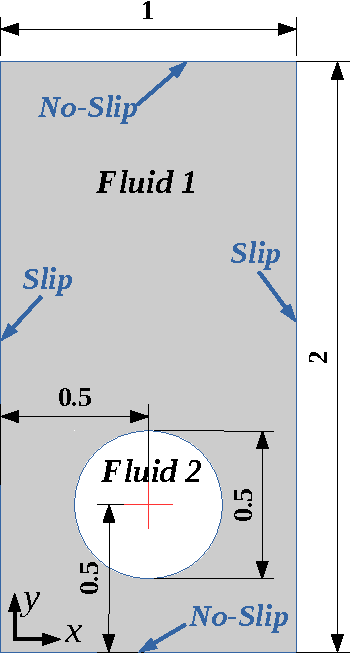
\includegraphics[width=4.25cm]{figures/benchmark_scheme.pdf}
 \vspace{-7mm}
\end{center}
\caption{Configuration and boundary conditions for 2D bubble benchmark.}
\label{fig:1}
\end{figure}
The 2D case setup is schematized in Figure~\ref{fig:1}. First phase (liquid) properties are 
$\rho_1=1000$ kg/m$^3$, $\mu_1=10$ kg/(ms), while second phase (gas) takes $\rho_2=1$ kg/m$^3$, $\mu_2=0.1$ kg/(ms) as physical parameters. 
The surface tension is $\sigma=1.96$ kg/s$^2$. Gravity is taken as $g=0.98$ m/s$^2$. Extension of the case to 3D is straightforward.

Square/cubic cells were used for all simulations in 2D/3D. Six grid resolutions have been used ranging from 20 to 640 cells along the $x$ direction, with the cell size halfed in each refinement. The bubble was initialized as a cylinder in 2D and as a sphere in 3D using the \verb+setFields+ utility. The Crank-Nicolson second order time scheme with blending coefficient 0.9 has been used for all computations. The convective term was treated with \verb+Gauss limited linearV 1+, and in the MULES simulations \verb+Gauss vanLeer+ was used for the $\alpha$ convection. The \verb+Gauss linear+ scheme was used for gradient terms. The GAMG implicit solver was used for pressure terms, while the smooth solver was used for the velocity. Constant time steps have been used, starting at $\Delta t=0.002$ s for the coarsest level and reduced for finer grids to keep the maximum CFL number below 0.05. The PIMPLE algorithm was run in PISO mode (\verb+nOuterCorretors+ set to 1) with 3 PISO correctors. Setting \verb+momentumPredictor+ to \verb+true+ was important for accuracy with isoAdvector. Computations were run up to time $t=3$ s in 2D and $t=3.5$ s in 3D. 

%%======================================================================
\section{Results}\label{sec_results}
%%======================================================================
Post-processing quantities of interest are described in details in~\cite{Hysing2009,Adelsberger2014}. These are the vertical position of the bubble centroid, the bubble rise velocity, the bubble circularity/sphericity, bubble area/volume and surface perimeter/area in 2D/3D. The circularity/sphericity is the inverse ratio of the bubble surface perimeter/area to the area/volume-equivalent circle/sphere in 2D/3D. It takes the value 1 at the beginning of the computation and decreases as the bubble deforms.
   
The Figure~\ref{fig:2} shows the bubble shape obtained with MULES and isoAdvector for the finest 2D simulation at time $t = 3$ s together with results from the reference data from ~\cite{Hysing2009}. Slight differences appear in the prediction of the front and back main interface positions (see zooms 1 and 2), with the most noticable difference being isoAdvector falling slightly behind the other methods. All the codes predict rather different trains of detached bubbles (see zoom 3 frame). The time evolution of Figure~\ref{fig:3} shows a comparison between MULES and isoAdvector at grid resolution 160, and for the 2D calculations. Again results are very similar, especially for the main bubble shape, and we see a small retardation of the isoAdvector bubble compared with the MULES bubble towards the end of the simulation.
\begin{figure}[!h]
  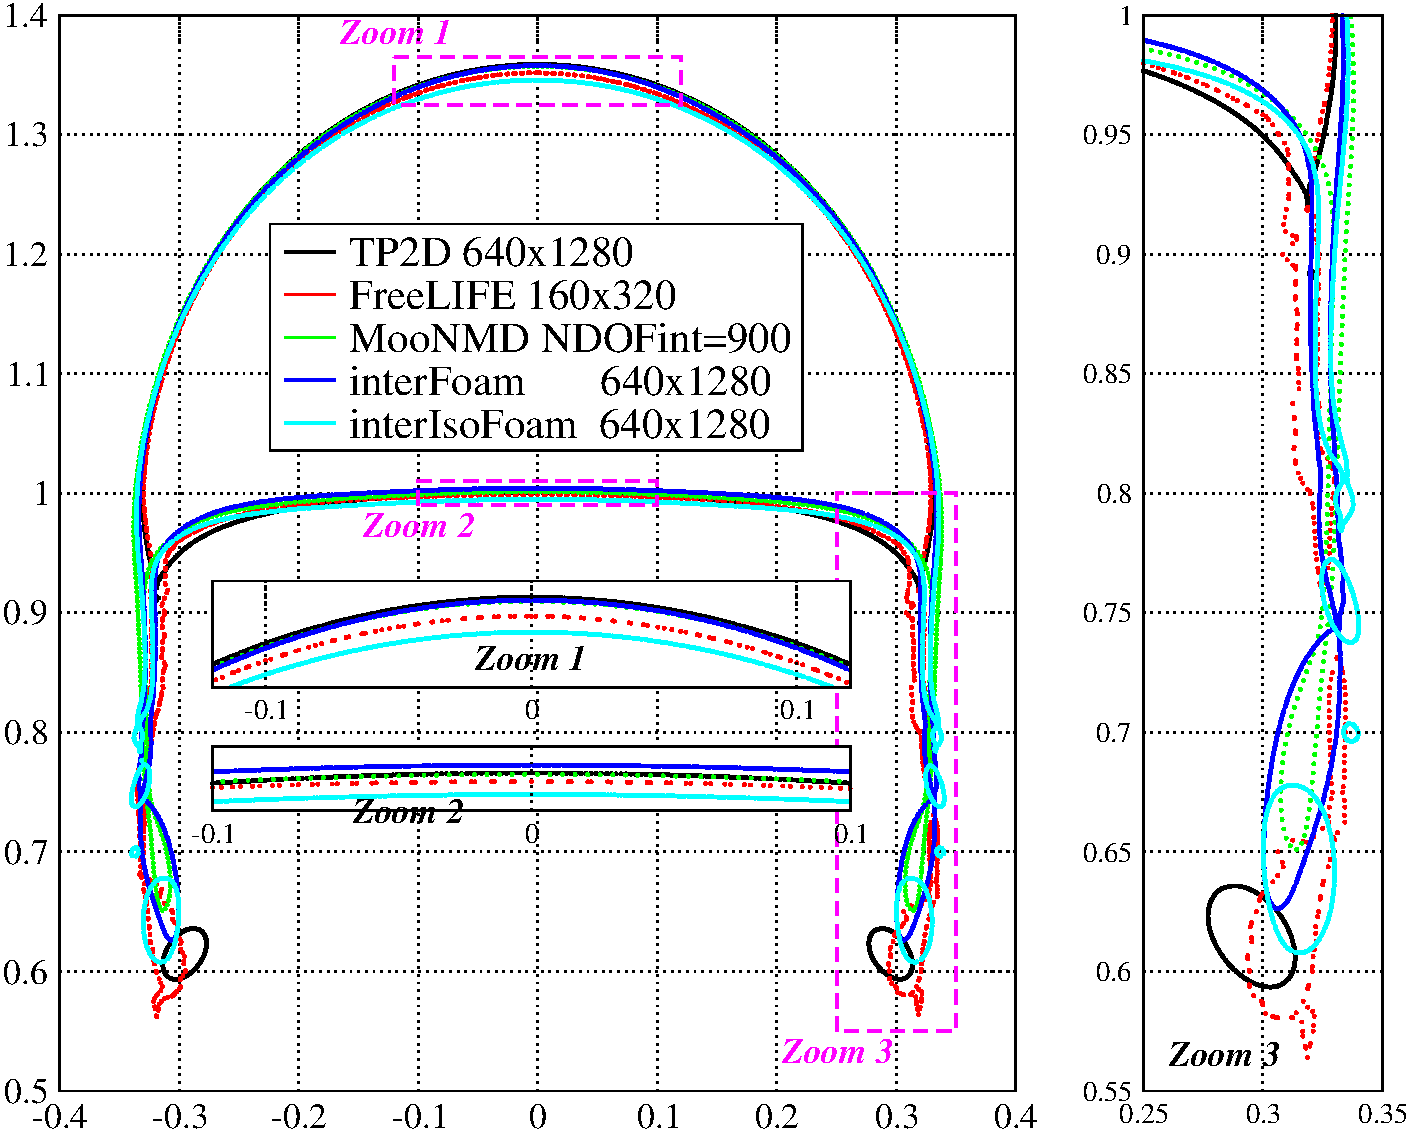
\includegraphics[scale=0.5]{figures/bubble_shape2D_t=3.pdf}
  \caption{Comparison of bubble shapes at final time $t=3$ s for 2D test case.}
  \label{fig:2}
\end{figure}

Figure~\ref{fig:4} shows 3D results for the rise velocity and sphericity. MULES and isoAdvector 
results are almost identical. When compared with the available reference data, the bubble rise velocity is, however, overpredicted by both solvers. 
This discrepancy will require further investigation, as the results obtained in reference~\cite{Adelsberger2014} using \verb+interFoam+ version 2.2.2 differ from the currently used version taken from OpenFOAM-v1712.
The right hand side of Figure~\ref{fig:4} shows that sphericity results start to differ between 
MULES and isoAdvector at times larger than roughly 2.5 s. This is mainly explained by the presence of small trains of detached bubbles in the isoAdvector run. The available reference data shows that the scatter between all the different solvers is important at large times. This is again explained by the prediction of different structures in the bubble queue, as observed in 2D 
(see also Figure~\ref{fig:2}).  
%\vspace{-2mm}
\begin{figure}[!h]
  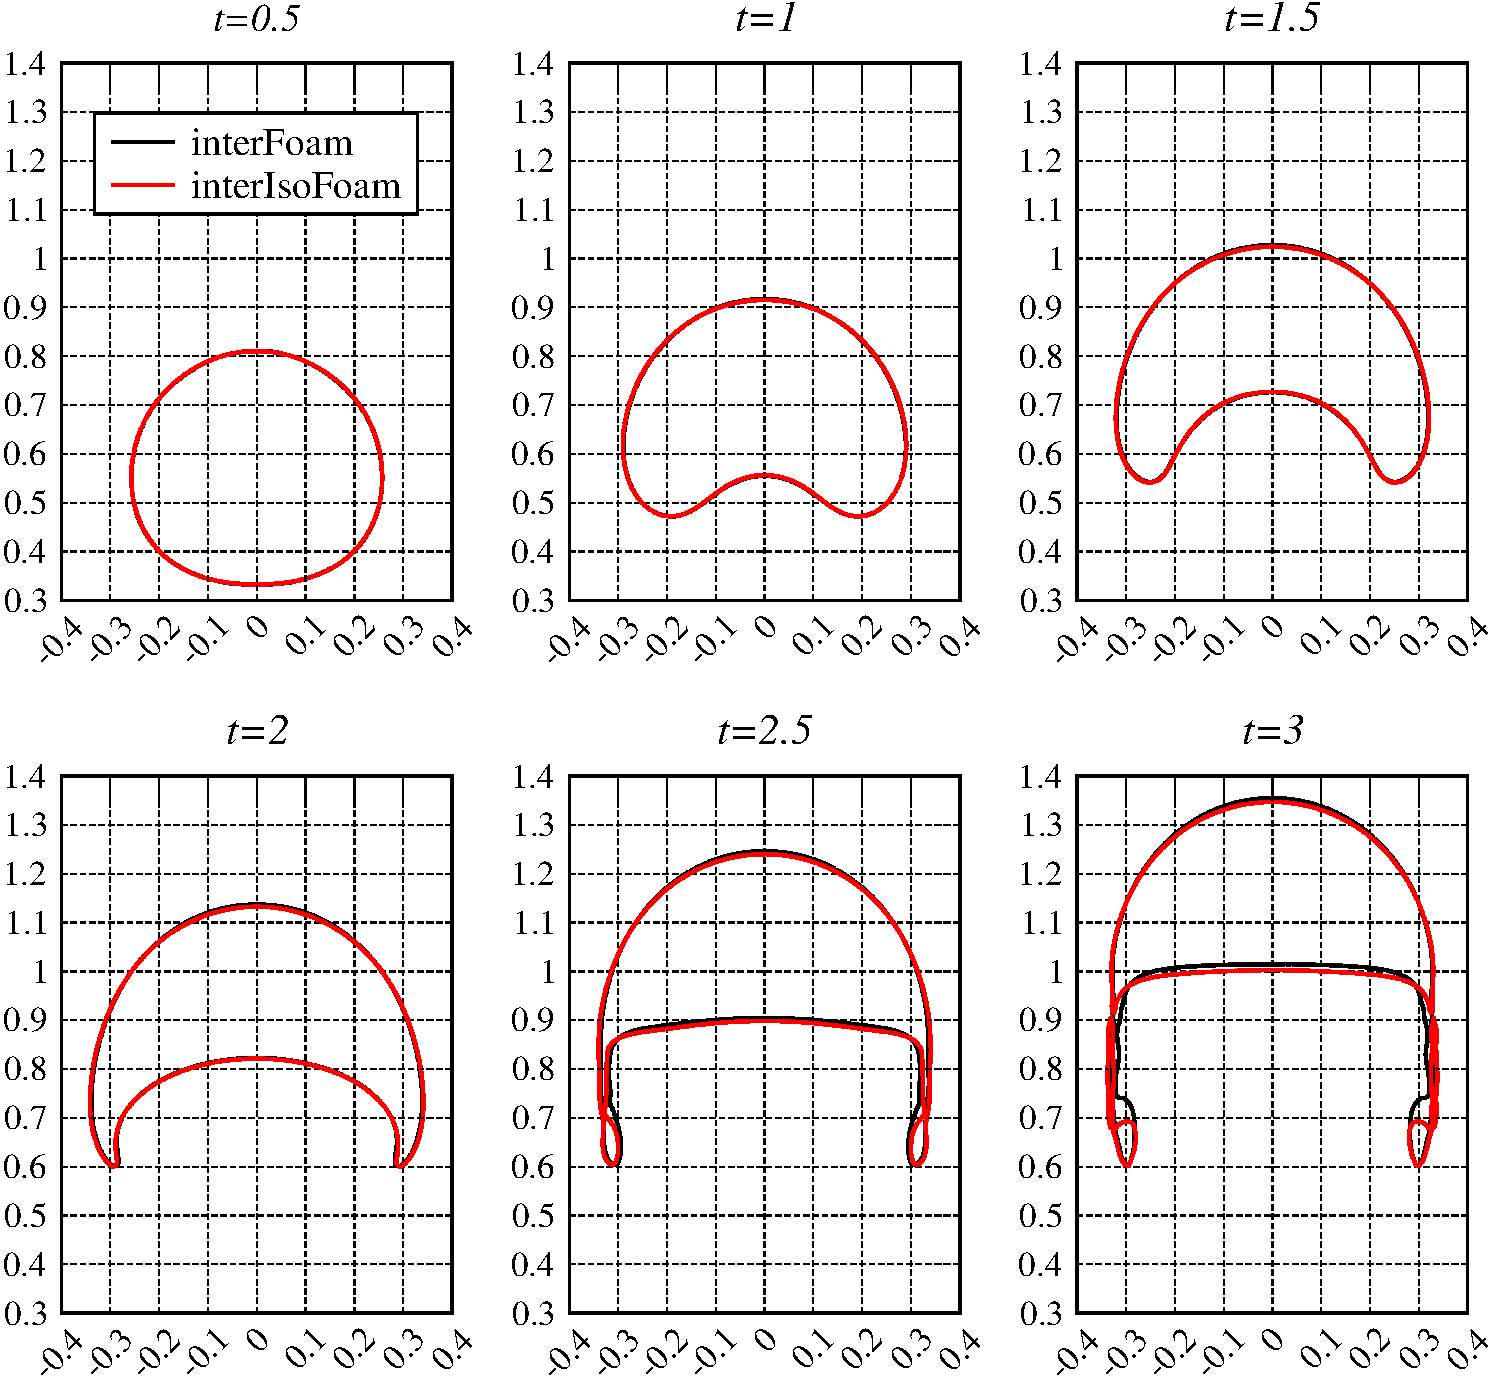
\includegraphics[scale=0.45]{figures/bubble_shape2D_time_evol_160.pdf}
  \caption{Time evolution of bubble shapes for 2D test case at resolution $160\times320$. 
           Comparison of MULES with isoAdvector.}
  \label{fig:3}
\end{figure}
%\vspace{-3mm}
\begin{figure}[!h]
  \centering
%  \vspace{-3mm}
  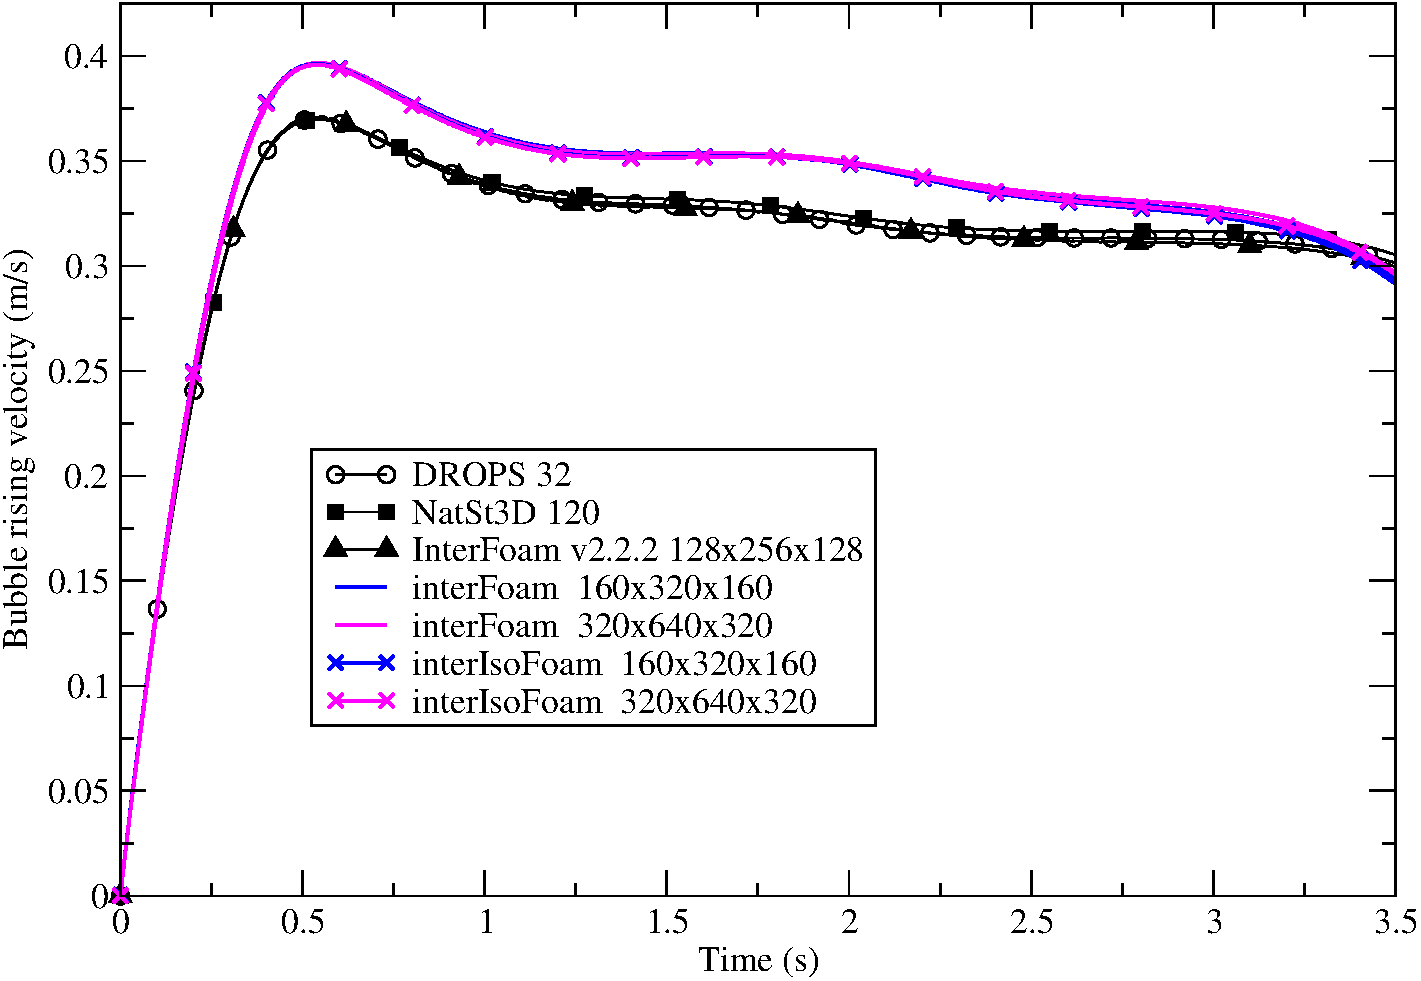
\includegraphics[scale=0.333]{figures/bubble_velocity3D.pdf}
  \hspace{0.8cm}
  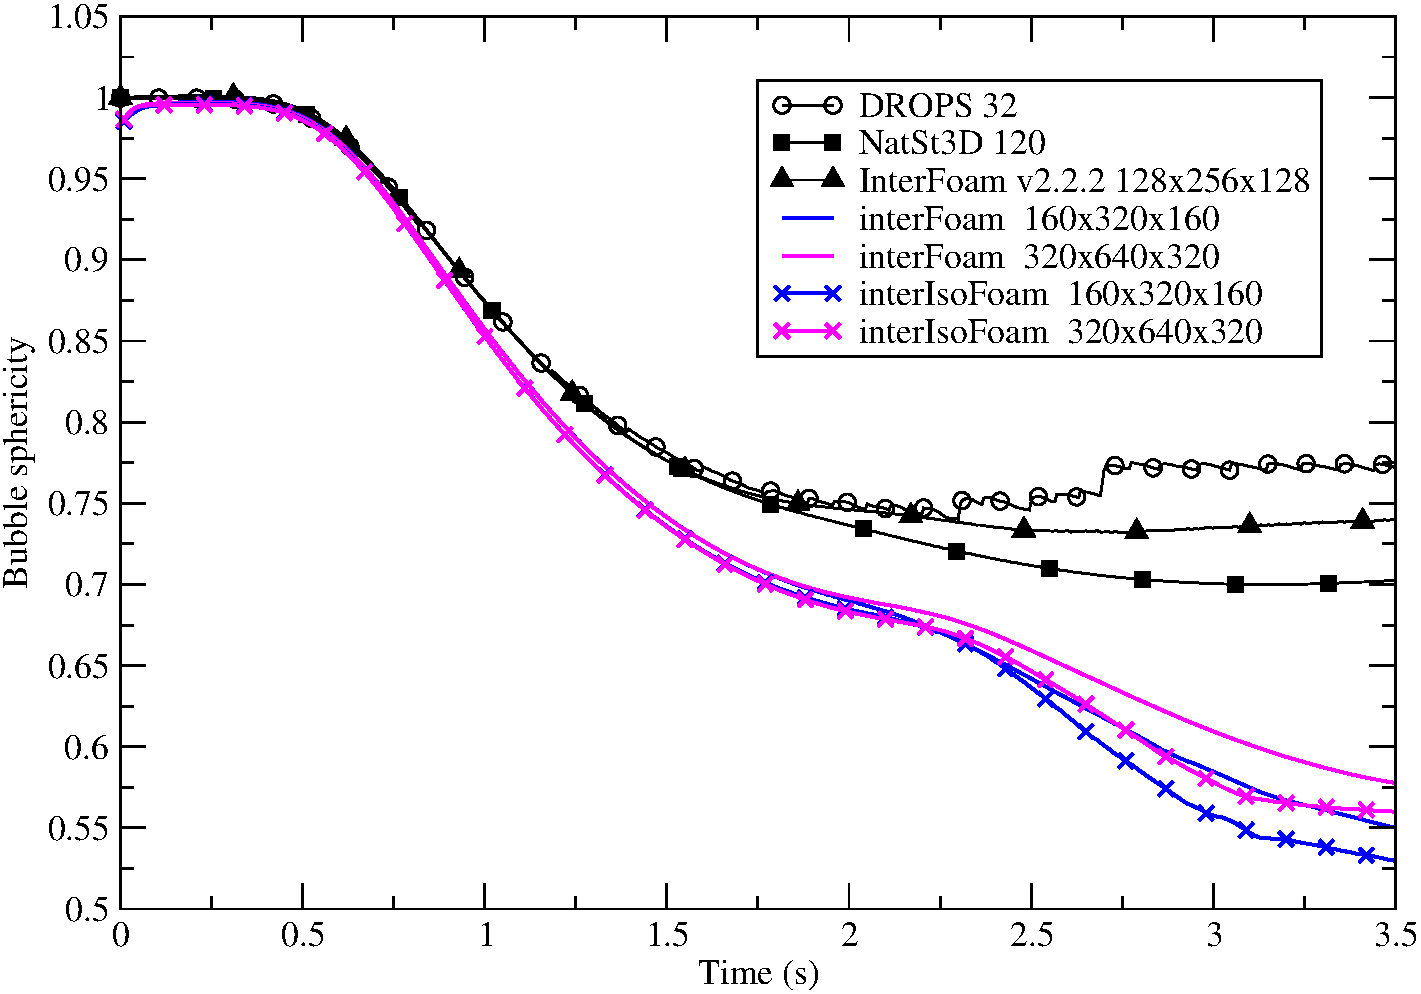
\includegraphics[scale=0.333]{figures/bubble_sphericity3D.pdf}
  \caption{Time evolution of rise velocity (left) and sphericity (right) for 3D test case. }
  \label{fig:4}
\end{figure}

3D computations have been run on the Occigen supercomputer at CINES, on Intel 
Xeon E5-2690V3. The largest computation with 
$320 \times 640 \times 320 = 65 536 000$ cells was run on 504 cores for 29.25 hours for
MULES versus 26.78 hours for isoAdvector (so about 10\% faster). 


\begin{figure}[!h]
\begin{center}
 \vspace{-1mm}
 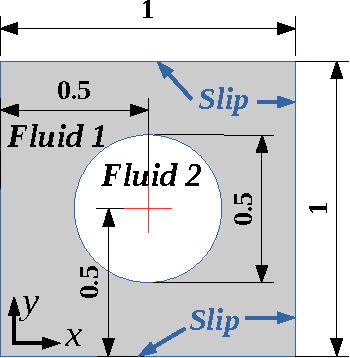
\includegraphics[width=4.25cm]{figures/spuriousCurrents_scheme.pdf}
 \vspace{-7mm}
\end{center}
\caption{Configuration and boundary conditions for 2D spurious currents test case.}
\label{fig:spuriousCurrents_scheme}
\end{figure}



\begin{figure}[!h]
\begin{center}
 \vspace{-1mm}
 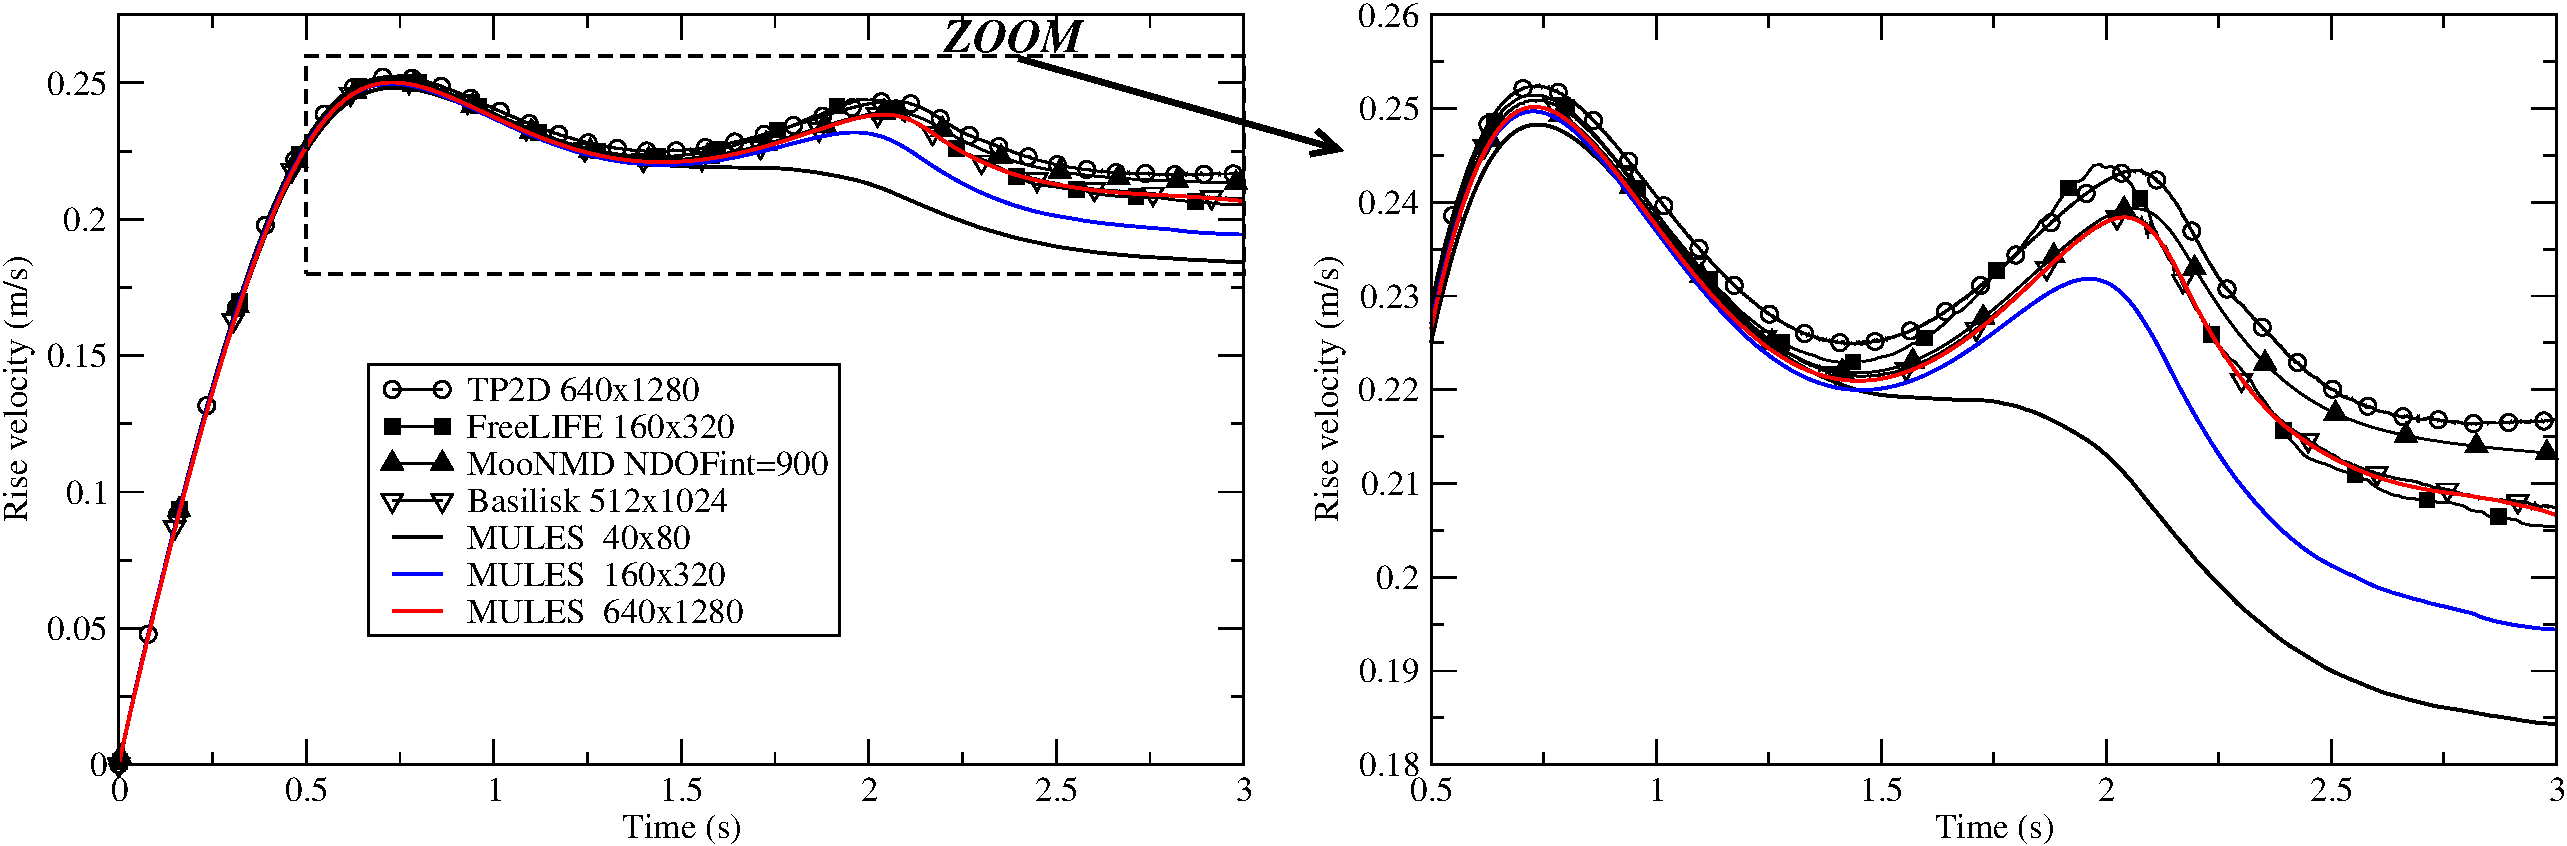
\includegraphics[width=\textwidth]{figures/HysingB_bubble_velocity_MULES.pdf}
 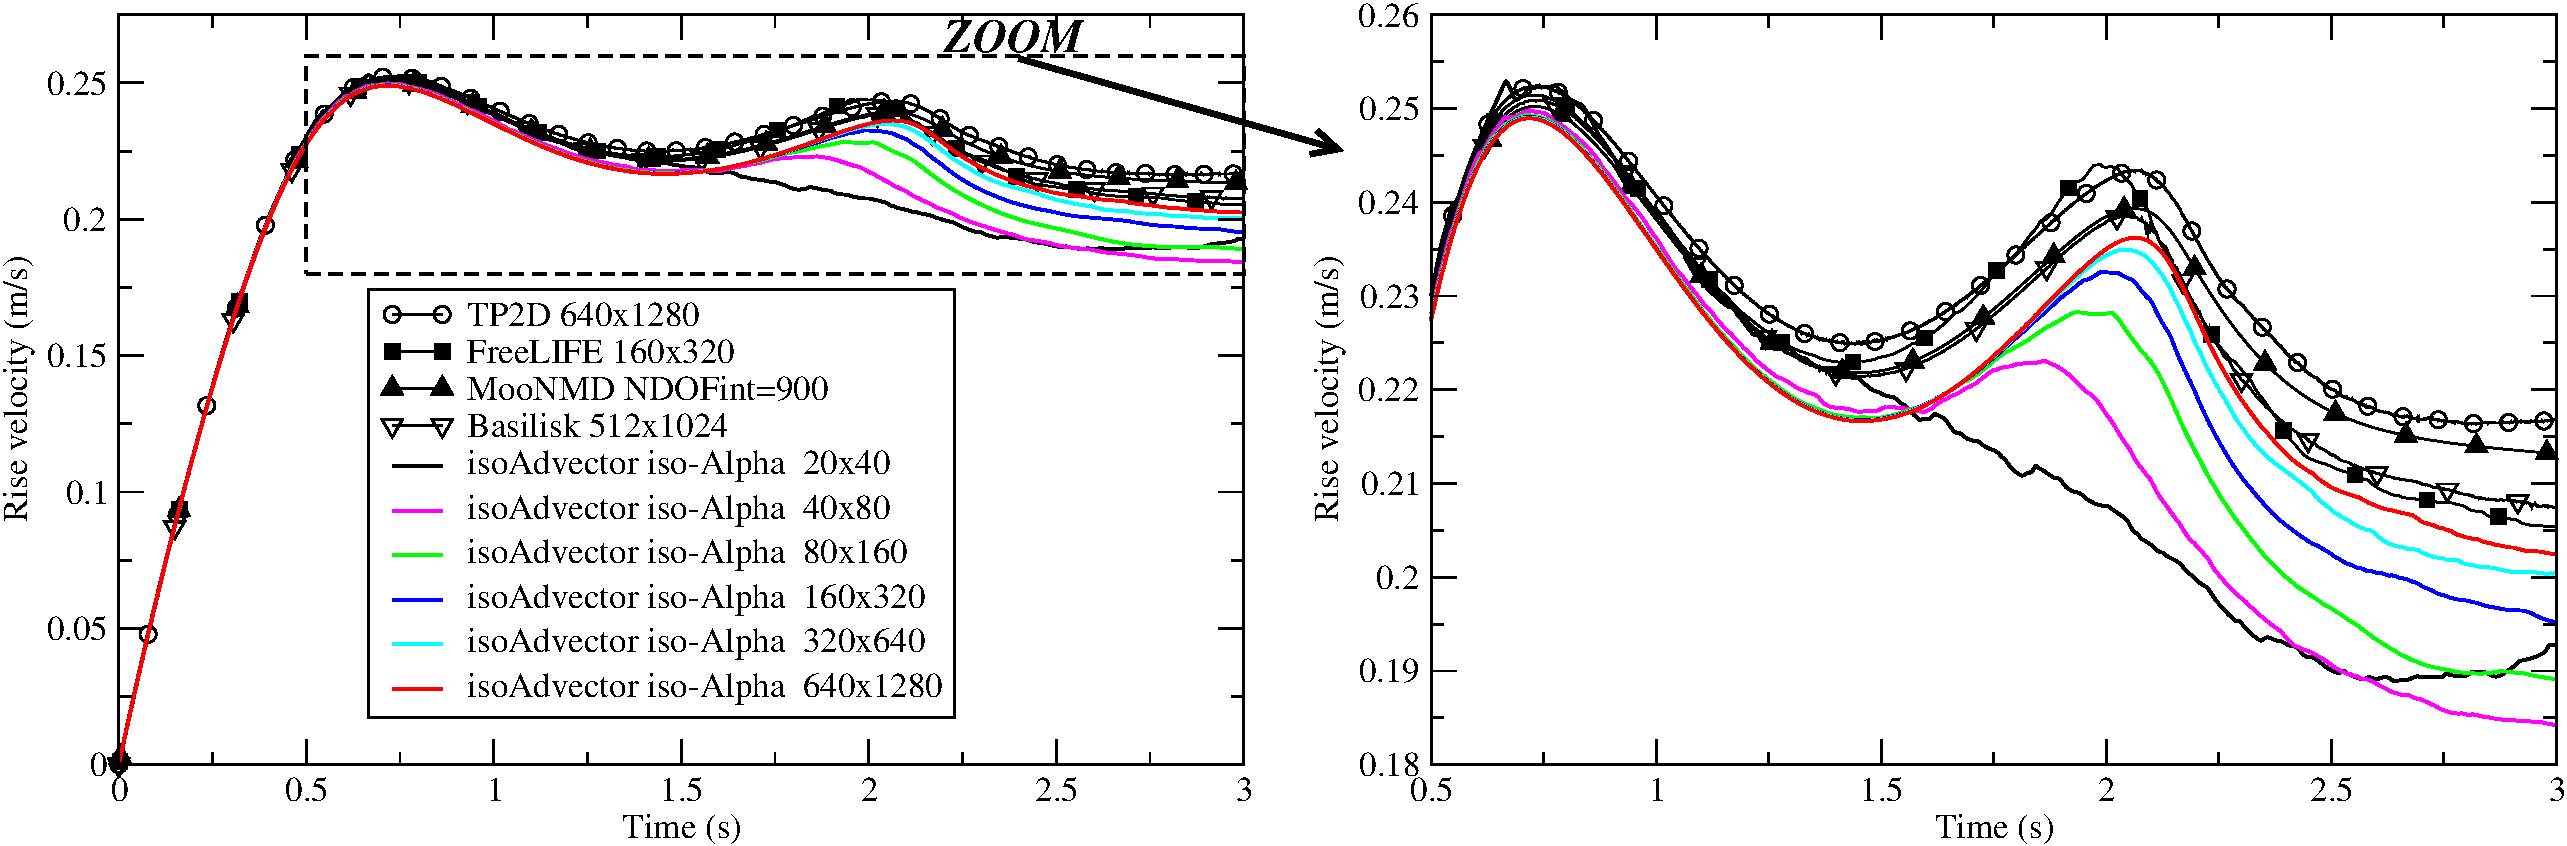
\includegraphics[width=\textwidth]{figures/HysingB_bubble_velocity_isoAlpha.pdf}
 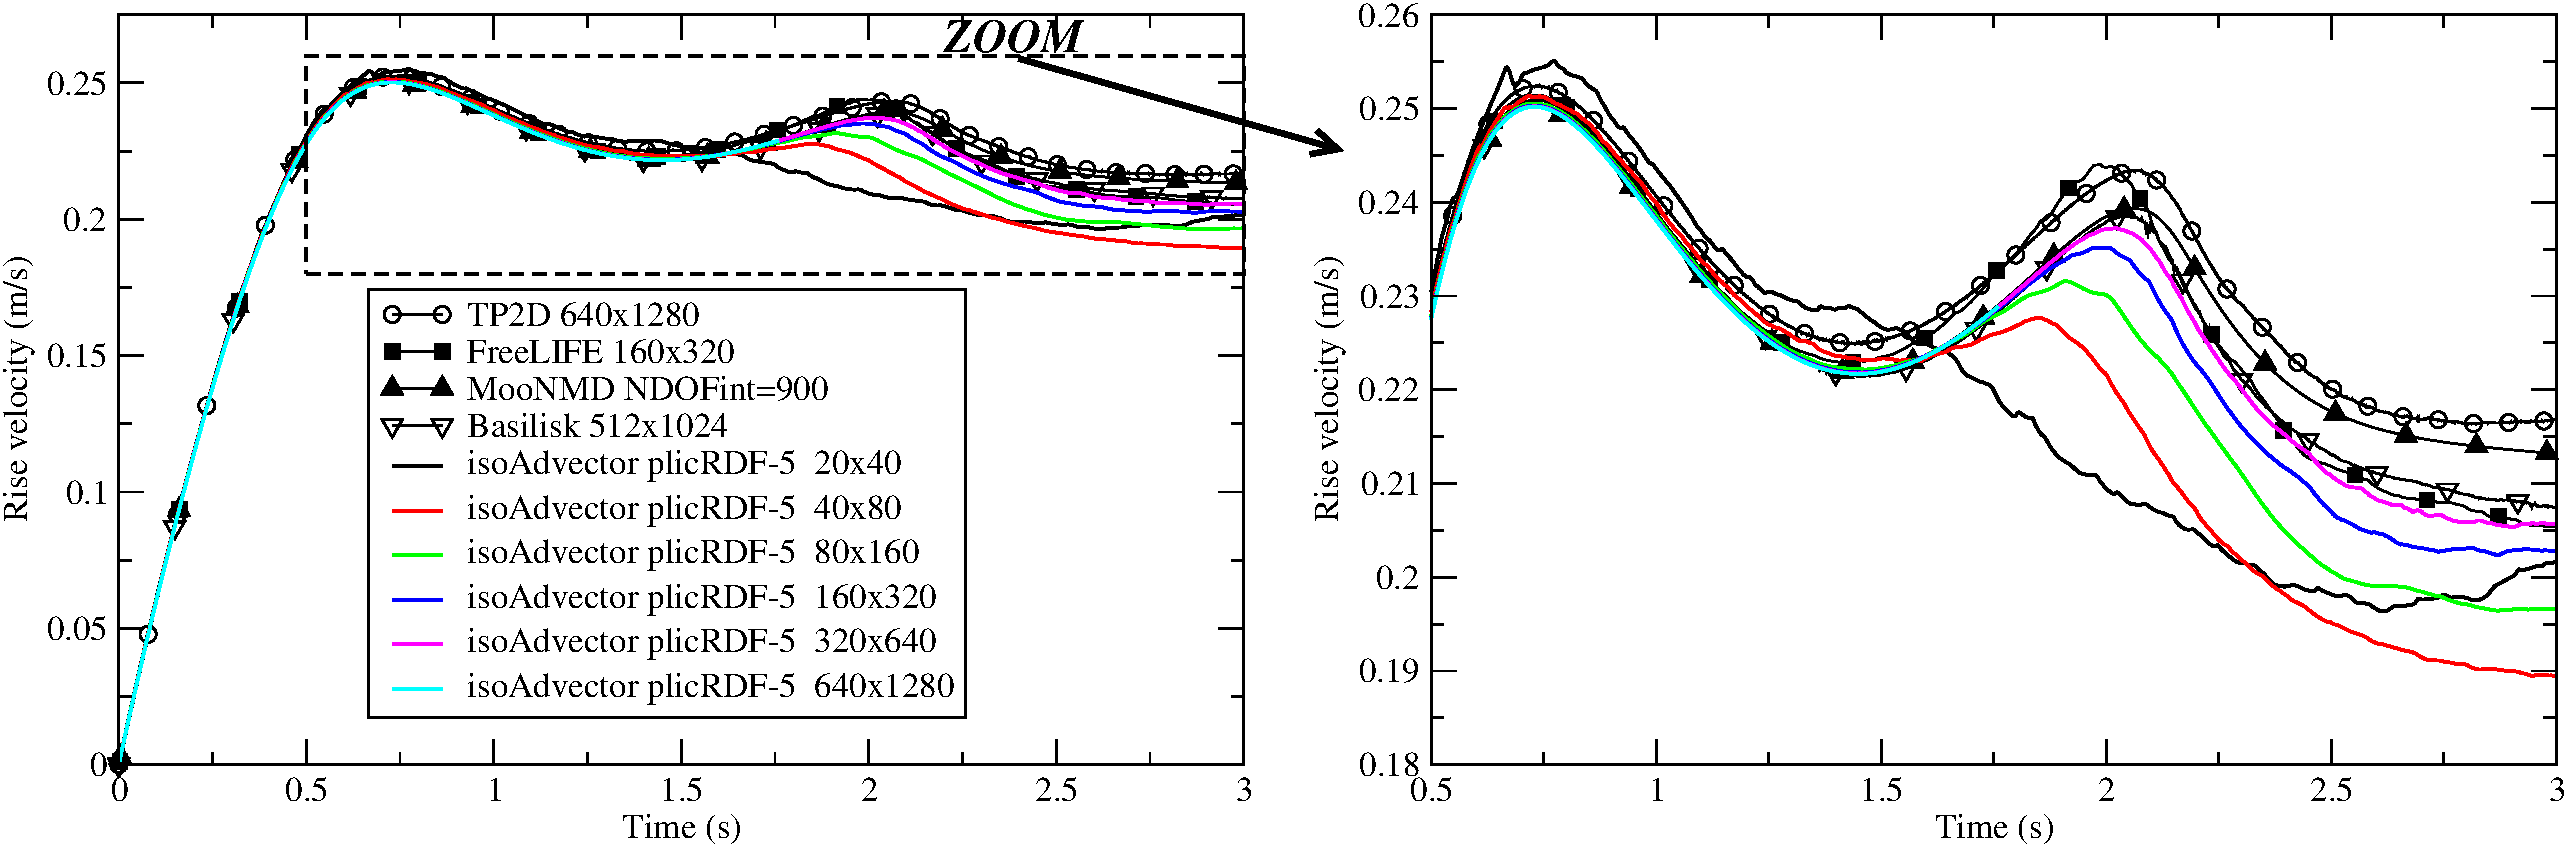
\includegraphics[width=\textwidth]{figures/HysingB_bubble_velocity_plicRDF5.pdf}
 \vspace{-14mm}
\end{center}
\caption{Time evolution of rise velocity on hexahedral grids for solvers MULES (top), isoAdvector with isoAlpha (middle) and plicRDF5 (botttom) reconstruction schemes.}
\label{fig:HB_Struct_bubble_velocity}
\end{figure}



\begin{figure}[!h]
\begin{center}
 \vspace{-1mm}
 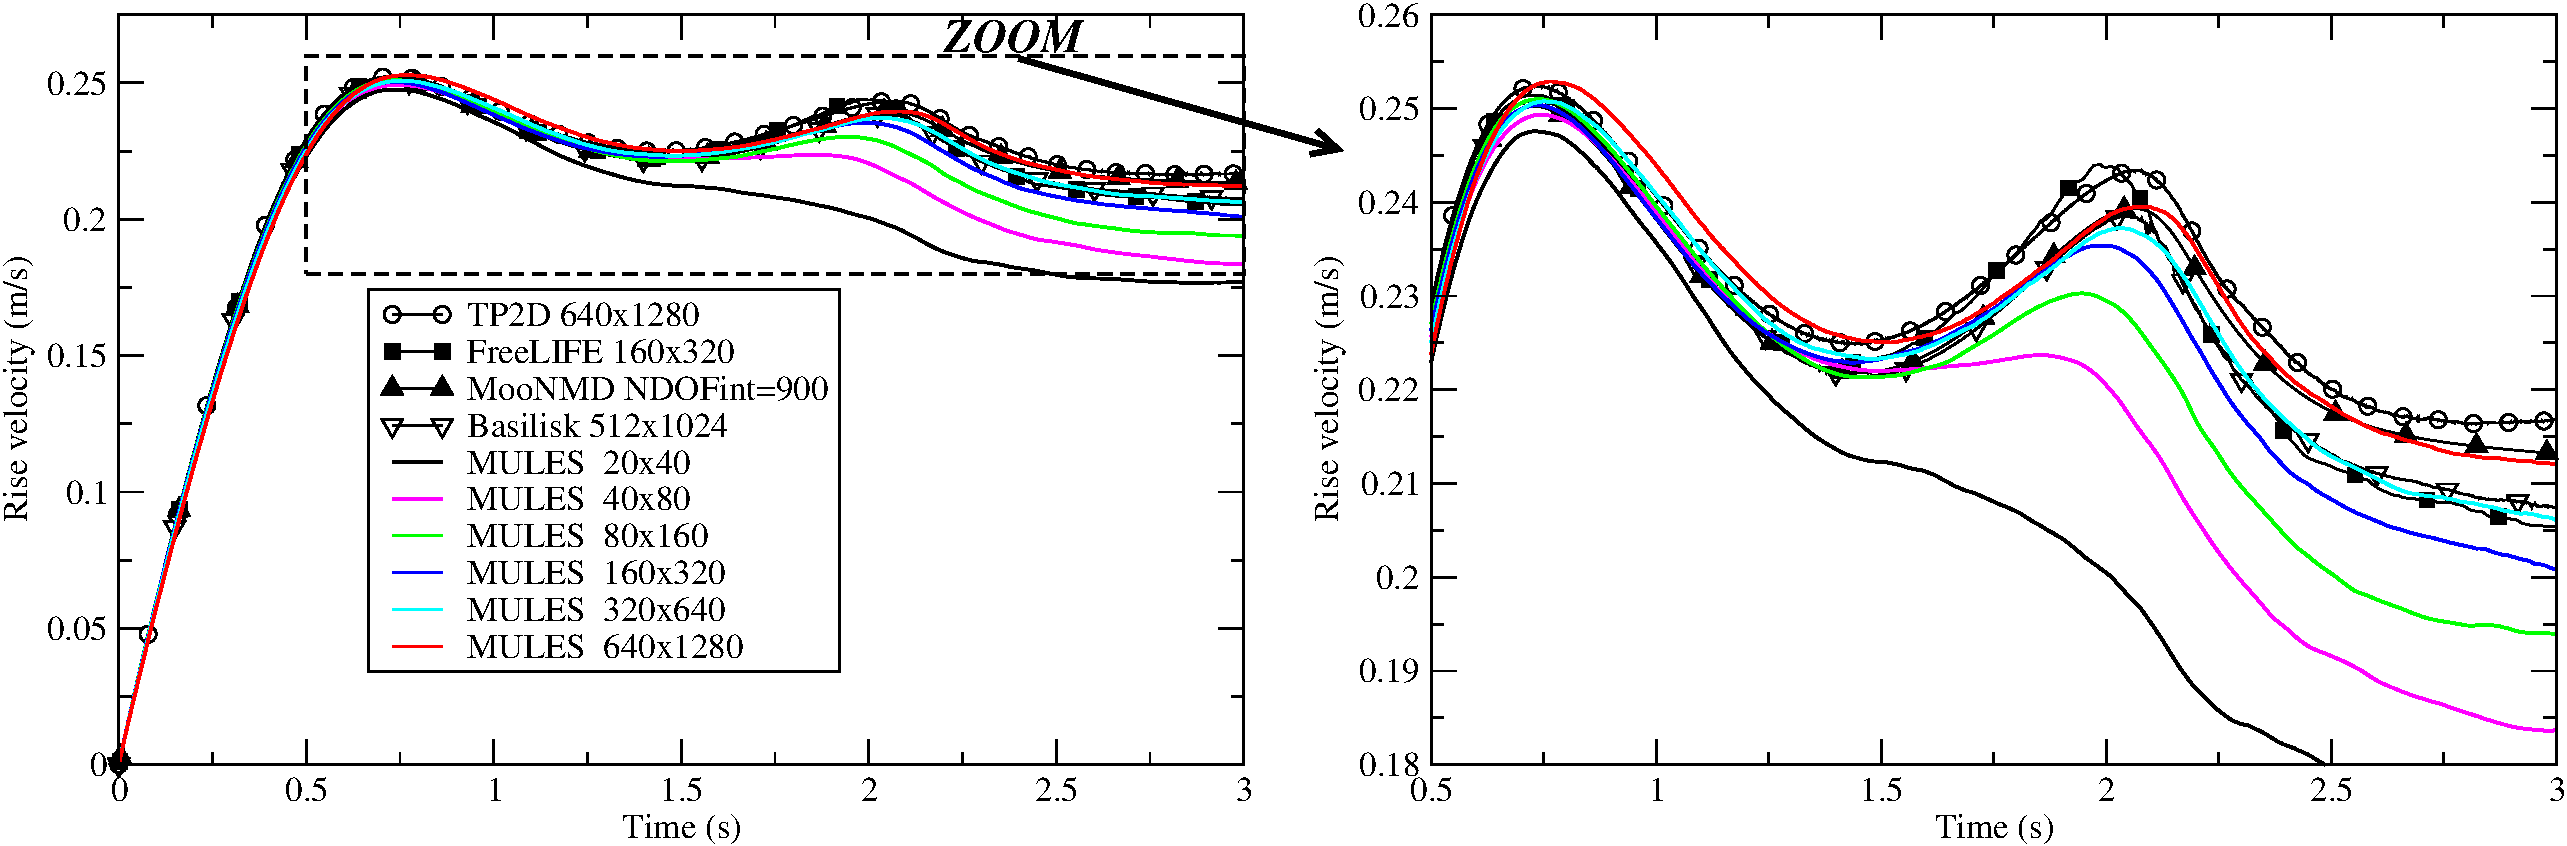
\includegraphics[width=\textwidth]{figures/HysingB-uns_bubble_velocity_MULES.pdf}
 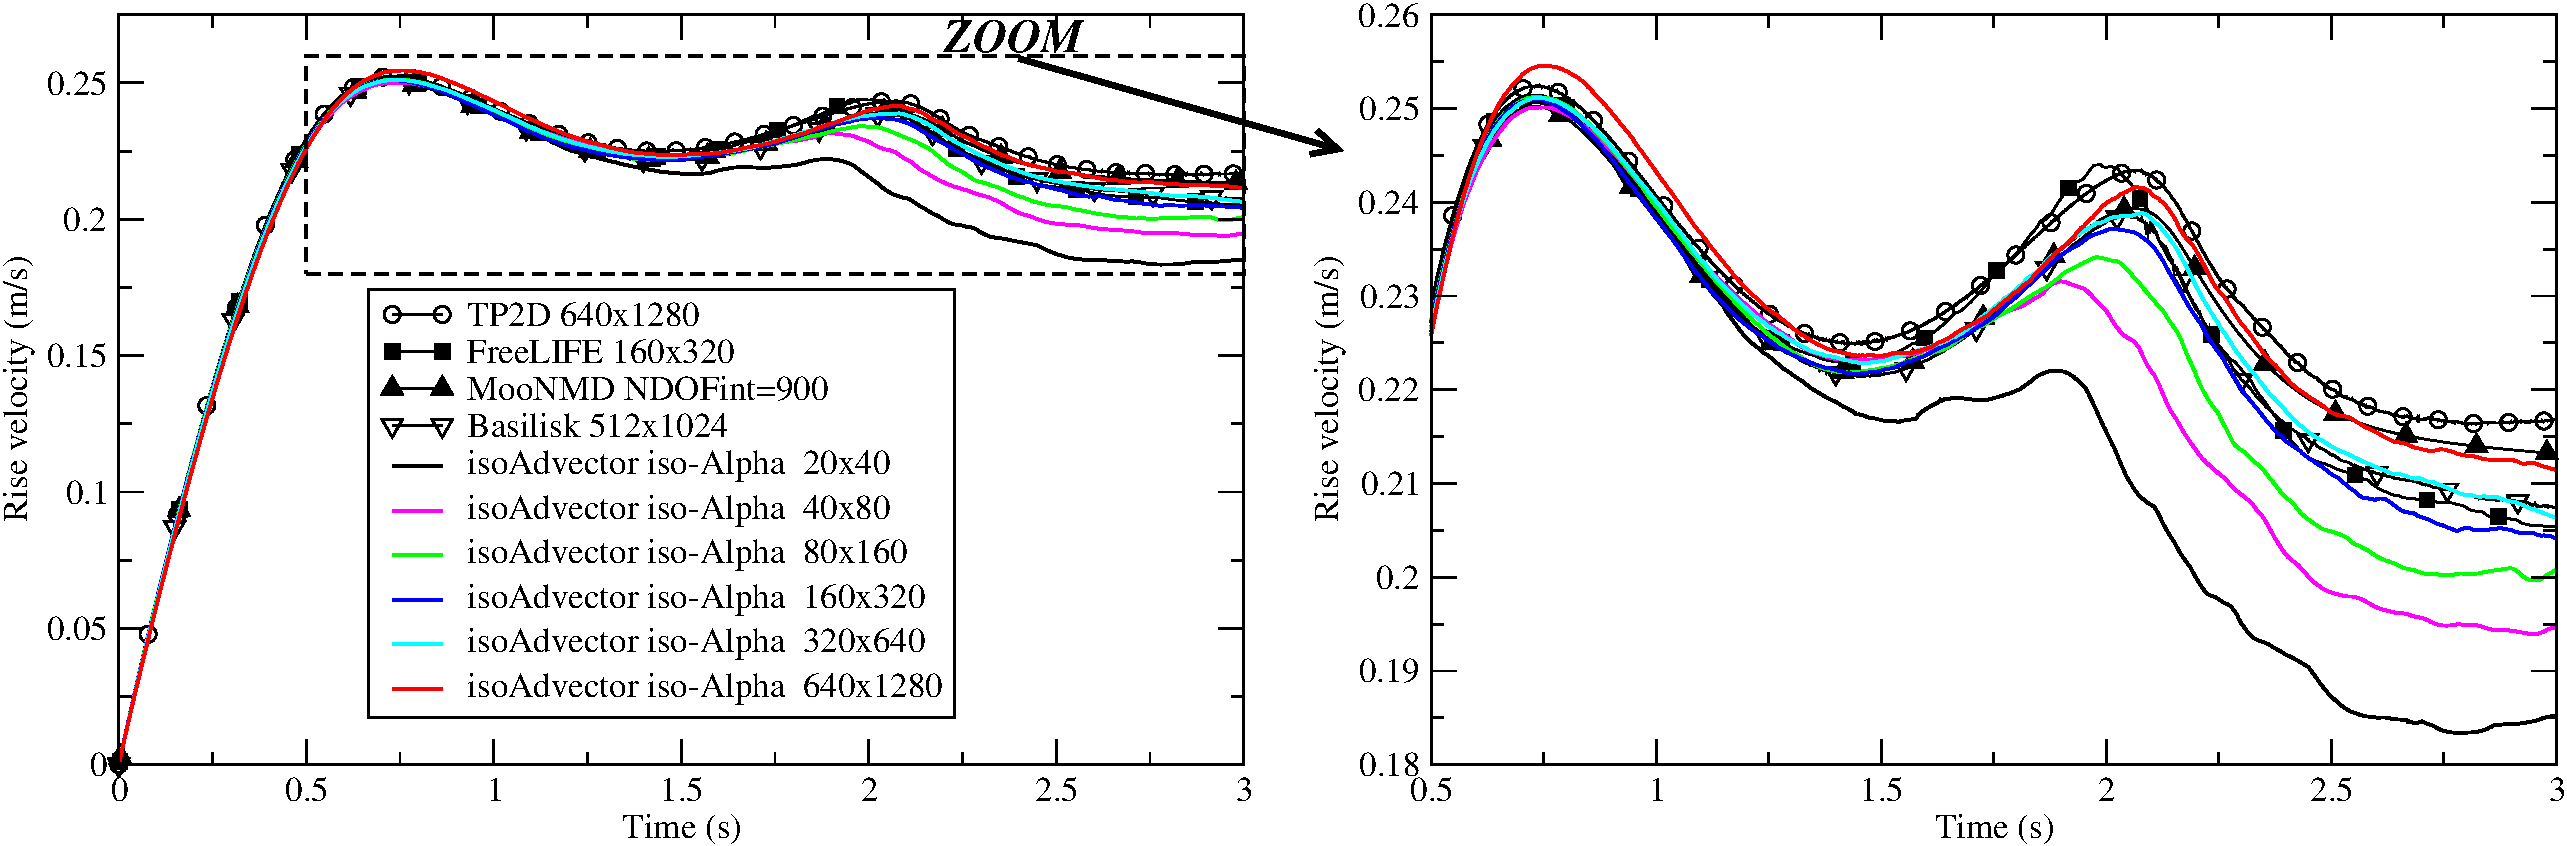
\includegraphics[width=\textwidth]{figures/HysingB-uns_bubble_velocity_isoAlpha.pdf}
 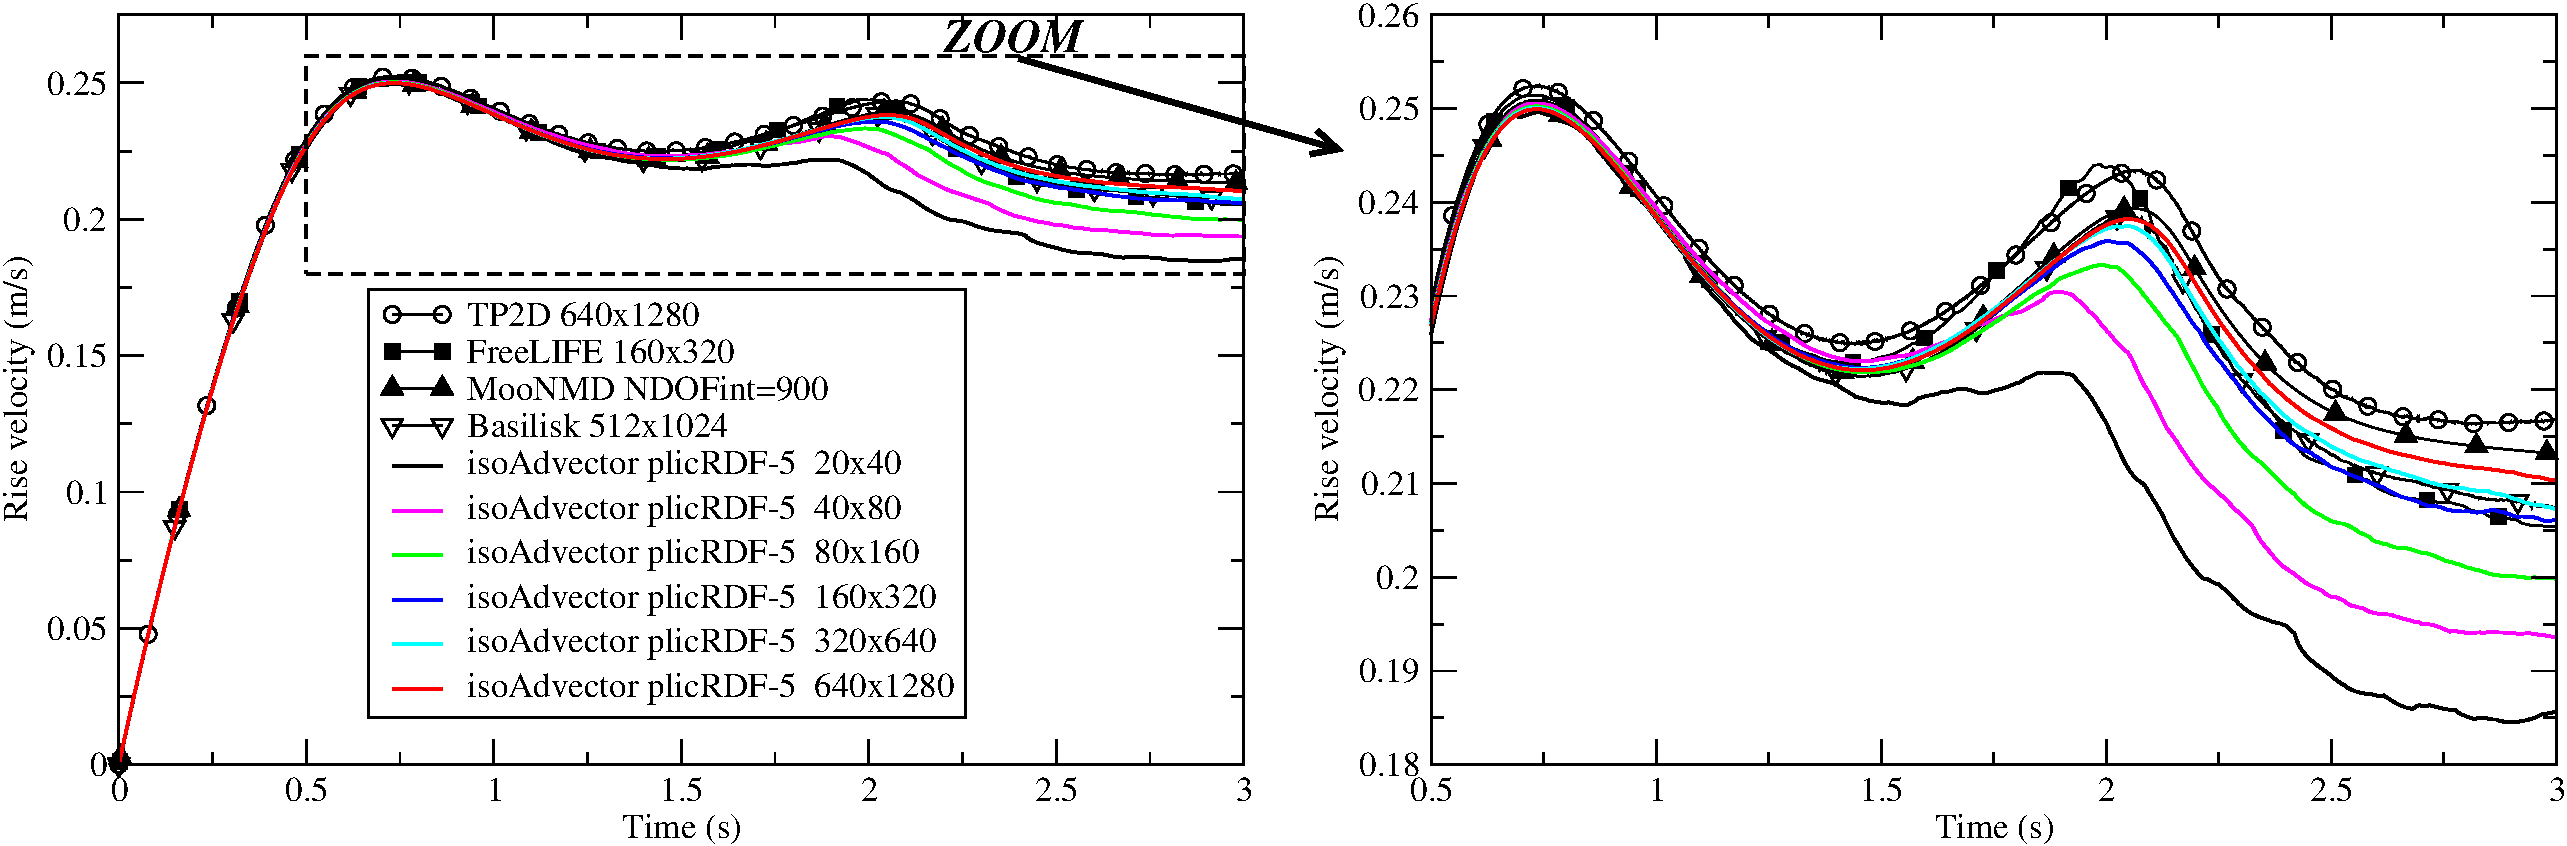
\includegraphics[width=\textwidth]{figures/HysingB-uns_bubble_velocity_plicRDF5.pdf}
 \vspace{-14mm}
\end{center}
\caption{Time evolution of rise velocity on triangular grids for solvers MULES (top), isoAdvector with isoAlpha (middle) and plicRDF5 (botttom) reconstruction schemes.}
\label{fig:HB_Uns_bubble_velocity}
\end{figure}


%%======================================================================
\section{\small Conclusion}
%%======================================================================
This paper has shown a quantitative validation of the isoAdvector method against MULES and other 
codes. The test case used is the Hysing benchmark, both in 2D and 3D. isoAdvector has been verified to work for rising bubble simulation with similar accuracy as MULES and with a sharper interface and slightly smaller calculation times.
This reference case will be contributed to the OpenFOAM\textsuperscript{\textregistered} tutorial wiki.

%%======================================================================
\section*{Acknowledgments}
%%======================================================================
\noindent
This  work  was  granted  access  to  the  HPC  resources  of CINES under the 
allocation 2018-AP012B10362 made by GENCI.

%%======================================================================
\section*{References}
%%======================================================================

\bibliography{references.bib}

\end{document}
